\documentclass[12pt, letterpaper]{article}

\usepackage[utf8]{inputenc}
\usepackage{graphicx}
\usepackage{parskip}
\usepackage{amsmath}
\usepackage{amssymb}
\usepackage[section]{placeins}
\usepackage{import}
\usepackage{xifthen}
\usepackage{pdfpages}
\usepackage{transparent}
\usepackage{gensymb}

\graphicspath{{../media/}}

\title{Modeling Pan and Tilt of Laser Mount}
\author{Nabeel Chowdhury}
\date{\today}

\newcommand{\incfig}[1]{%
    \def\svgwidth{\columnwidth}
    \import{../media/}{#1.pdf_tex}
}

\begin{document}
	\maketitle
	\newpage
	
	\section{Description of Laser Mount Measurements}
		\begin{figure}[ht]
			\centering
			\resizebox{0.58\textwidth}{!}{\incfig{LaserMountDiagram}}
			\caption{\textbf{A} is the height of the panning arm and \textbf{$\theta_1$} is the rotation of the panning arm. \textbf{B} is the offset distance of the tilting arm. It is perpendicular to the panning arm. \textbf{C} is the length of the tilting arm. \textbf{D} is the distance of the base of the tilting arm to the target. This distance changes with panning angle, but stays constant with tilt.}
		\end{figure}
	
	\newpage
	\section{Finding Tilt Angle}
		\subsection{Laser Hit above A and Below Horizontal}
			\begin{figure}[ht]
				\centering
				\resizebox{0.7\textwidth}{!}{\incfig{Shallow Obtuse}}
				\caption{\textbf{D} is target's distance from the base of the tilting arm. \textbf{E} is the height above the base of the tilting arm that the laser hits its target. \textbf{a} is the hypotenuse of the extended triangle from the extrapolated intersection of the laser with the level of the base of the tilting arm. \textbf{b} is the hypotenuse of the extended triangle minus the distance of the base of the tilting arm to the target.}
			\end{figure}
			
			\newpage
			In order to find the height of the height of the target hit location, \textbf{E}, we need to find \textbf{b}.
			
			\begin{flalign*}
				b &= a-D &\\
				a &= \frac{C}{\sin(\theta_2 - 90 \degree)} = \frac{C}{-\cos(\theta_2)} &\\
				\therefore b &= -\frac{C}{\cos(\theta_2)} + D &\\
				-\frac{\textbf{E}}{\frac{C}{\cos(\theta_2)} + D} &= \tan(\theta_2 - 90 \degree) = -\cot(\theta_2)&\\
				\therefore \textbf{E} &= \left[D + \frac{C}{\cos(\theta_2)} \right] \cot(\theta_2) = D \cot(\theta_2) + \frac{C}{\sin(\theta_2)}&\\
			\end{flalign*}
			
			Now assuming we want to input in a target height to hit, we need to extract $\theta_2$ from the equation.
			
			\begin{flalign*}
				\text{If } x &= \tan(\frac{\theta_2}{2})\text{, } \sin(\theta_2) = \frac{2x}{1 + x^2}\text{, } \cos(\theta_2) = \frac{1 - x^2}{1 + x^2}\text{, } \tan(\theta_2) = \frac{2x}{1-x^2}&\\
				\textbf{E} &= D \frac{1-x^2}{2x} + C \frac{1 + x^2}{2x} &\\
				2\textbf{E}x &= D (1-x^2) + C (1 + x^2) &\\
				0 &= \left(C - D \right) x^2 - 2\textbf{E}x + C + D &\\
				x &= \frac{2\textbf{E} \pm \sqrt{4\textbf{E}^2 - 4\left( C - D \right)}}{2 \left( C - D \right)} = \tan(\frac{\theta_2}{2}) &\\
				&\therefore \boxed{\theta_2 = 2 \tan^{-1} \left[ \frac{2\textbf{E} \pm \sqrt{4\textbf{E}^2 - 4\left( C - D \right)}}{2 \left( C - D \right)} \right]} &\\
			\end{flalign*}
			
			The actual value of $\theta_2$ is the positive angle that results from the inverse tangent calculation.
			
		\subsection{Laser Hit above A and Above Horizontal}
			\begin{figure}[ht]
				\centering
				\resizebox{0.7\textwidth}{!}{\incfig{Acute}}
				\caption{\textbf{D} is target's distance from the base of the tilting arm. \textbf{E} is the height above the base of the tilting arm that the laser hits its target. \textbf{a} is the hypotenuse of the smaller extended triangle from the extrapolated intersection of the laser with the level of the base of the tilting arm.}
			\end{figure}
			
			In order to find $\theta_2$, we first need to find \textbf{E}.
			\begin{flalign*}
				a &= \frac{C}{\cos(\theta_2)} &\\
				\therefore \textbf{E} & = \frac{D + a}{\tan(\theta_2)} = \frac{D + \frac{C}{\cos(\theta_2)}}{\tan(\theta_2}&\\
				\textbf{E} &= D \cot(\theta_2) + \frac{C}{\sin(\theta_2)}&\\
			\end{flalign*}
			
			This is the same result as the previous calculation. Therefore,
			\begin{flalign*}
				\theta_2 = 2 \tan^{-1} \left[ \frac{2\textbf{E} \pm \sqrt{4\textbf{E}^2 - 4\left( C - D \right)}}{2 \left( C - D \right)} \right]
			\end{flalign*}
			
		\subsection{Laser Hit below A}
			\begin{figure}[ht]
				\centering
				\resizebox{0.58\textwidth}{!}{\incfig{Deep Obtuse}}
				\caption{\textbf{D} is target's distance from the base of the tilting arm. \textbf{E} is the height below the base of the tilting arm that the laser hits its target. \textbf{a} is the distance from the base of the tilting arm to where the laser crosses the horitontal axis with respect to the base of the tilting arm. It is also the hypotenuse of the triangle made by the tilting arm and the laser crossing the horizontal made by the base of the tilting arm. \textbf{b} is the distance from the crossing to the target wall.}
			\end{figure}
			
			\newpage
			Once again, we need to find \textbf{E} based on the tilt angle.
			\begin{flalign*}
				b &= D - a &\\
				a &= \frac{C}{\cos(180 \degree - \theta_2)} = -\frac{C}{\cos(\theta_2)}&\\
				\textbf{E} &= \frac{b}{\tan(180 \degree - \theta_2)} = \frac{D + \frac{C}{\cos(\theta_2)}}{\tan(180 \degree - \theta_2)} = -\frac{\frac{C}{\cos(\theta_2)} + D}{\tan(\theta_2)} &\\
				\textbf{E} &= -\frac{C}{\sin(\theta_2)} - D \cot(\theta_2) &\\
			\end{flalign*}
			
			Solving for $\theta_2$:
			\begin{flalign*}
				\text{If } x &= \tan(\frac{\theta_2}{2})\text{, } \sin(\theta_2) = \frac{2x}{1 + x^2}\text{, } \cos(\theta_2) = \frac{1 - x^2}{1 + x^2}\text{, } \tan(\theta_2) = \frac{2x}{1-x^2}&\\
				\textbf{E} &= -C \frac{1 + x^2}{2x} - D \frac{1-x^2}{2x}&\\
				2\textbf{E}x &= -C (1 + x^2) - D (1-x^2)&\\
				0 &= \left(C - D \right) x^2 + 2\textbf{E}x + C + D &\\
			\end{flalign*}
			
			If we define E as negative when below the horizontal made by the base of the tilting arm, we get the same result as previously where.
				\begin{flalign*}
				\theta_2 = 2 \tan^{-1} \left[ \frac{2\textbf{E} \pm \sqrt{4\textbf{E}^2 - 4\left( C - D \right)}}{2 \left( C - D \right)} \right]
			\end{flalign*}
	
	\newpage		
	\section{Finding Pan Angle}
		\begin{figure}[ht]
			\centering
			\resizebox{0.9\textwidth}{!}{\incfig{Pan}}
			\caption{\textbf{B} is the length of the base of the tilting arm. \textbf{D} is target's distance from the base of the tilting arm. \textbf{F} horizontal distance of the target from center. \textbf{G} is the target's perpendicular distance from the panning arm.}
		\end{figure}
		
		Solving for $\theta_1$:
		\begin{flalign*}
			\tan(\theta_1) &= \frac{F}{G} &\\
			& \boxed{\therefore \theta_1 = \tan^{-1}(\frac{F}{G})} &\\
		\end{flalign*}
			
		\textbf{D} is a different distance now that the arm has panned. To find the new distance of D needed in the tilt angle calculations, we do the following:
		\begin{flalign*}
			\cos(\theta_1) &= \frac{G}{D + B} &\\
			D &= \frac{G}{\cos(\theta_1)} - B &\\
		\end{flalign*}
		
	\section{Creating a Model of the Laser Mount}
		\subsection{Creating the Default Position}
			In order to model how the tilt and pan angles will affect laser placement on the target and to debug issues while excluding hardware issues, I made a virtual model of the laser mount.
			
			Each segment of the model is oriented along the z axis first and then the pan and tilt local angles are applied. The angles between the base of the tilt arm and the pan arm and the laser with the tilt arm are set as $-90 \degree$.
			
			In this position, the pan angle turns the laser to the left and a positive tilt angle is subtracted from $180 \degree$. In the default position shown below, the tilt angle is $90 \degree$.
			
			\begin{figure}[ht]
				\centering
				\resizebox{0.9\textwidth}{!}{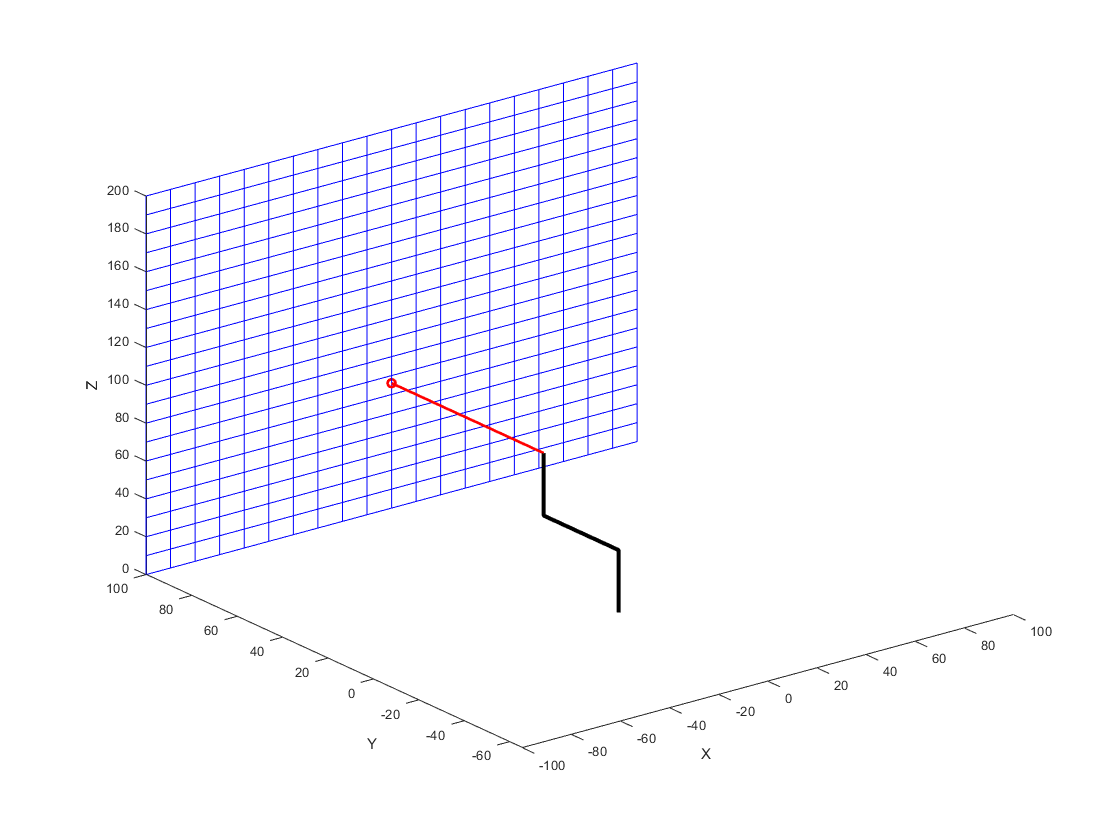
\includegraphics[scale=0.5]{defaultPosition}}
				\caption{The default position of the laser mount.}
			\end{figure}
		
		\subsection{Applying Local Rotations}
			When applying the tilt and pan angles, they need to be applied as local rotations and converted to the global positioning of the points that define the laser mount.
			\subsubsection{Rotation Matrices}
				The rotation matrices are below:
				
				\textbf{Rotation About the X Axis}
				\begin{equation*}
				R_x = 
					\begin{bmatrix}
						&1 &0 &0 \\
    					&0 &\cos(\theta) &\sin(\theta) \\
    					&0 &-\sin(\theta) &\cos(\theta)
					\end{bmatrix}
				\end{equation*}
				
				\textbf{Rotation About the Y Axis}
				\begin{equation*}
				R_y = 
					\begin{bmatrix}
						&\cos(\theta) &0 &-\sin(\theta) \\
    					&0 &1 &0 \\ 
    					&\sin(\theta) &0 &\cos(\theta)
					\end{bmatrix}
				\end{equation*}
				
				\textbf{Rotation About the Z Axis}
				\begin{equation*}
				R_z = 
					\begin{bmatrix}
						&\cos(\theta) &\sin(\theta)&0 \\
    					&\-sin(\theta) &\cos(\theta) &0 \\
    					&0 &0 &1
					\end{bmatrix}
				\end{equation*}
			
			\subsubsection{Matrix Multiplication}
				Matrix multiplication is done starting from the origin, which is the base of the panning arm, and then working out towards the each point of the mount to the end of the laser. Each new rotation is applied to the left of the previous rotations. The rotated location of each point is found by inverting the combined rotation matrices and multiplying it by the length of the segment. The new point then needs to be translated by the value of the previous point. 
				
				\textbf{Rotating the Panning Arm}
				\begin{flalign*}
					\begin{bmatrix}
						&x_P \\
						&y_P \\
						&z_P
					\end{bmatrix} &= R_z^{-1}(\theta_1)					
					\begin{bmatrix}
						&0 \\
						&0 \\
						&A
					\end{bmatrix} &\\
				\end{flalign*}
				
				\textit{Note that this rotation will always return the same position as the panning arm is align along the z axis at the origin.}
				
				\textbf{Rotating the Base of the Tilt Arm}
				\begin{flalign*}
					\begin{bmatrix}
						&x_B \\
						&y_B \\
						&z_B
					\end{bmatrix} &= (R_x(-90 \degree) R_z(\theta_1))^{-1}				
					\begin{bmatrix}
						&0 \\
						&0 \\
						&B
					\end{bmatrix} + 
					\begin{bmatrix}
						&x_P \\
						&y_P \\
						&z_P
					\end{bmatrix} &\\
				\end{flalign*}		
				
				\textbf{Rotation of the Tilt Arm}
				\begin{flalign*}
					\begin{bmatrix}
						&x_T \\
						&y_T \\
						&z_T
					\end{bmatrix} &= (R_x(\theta_2)R_x(-90 \degree) R_z(\theta_1))^{-1}				
					\begin{bmatrix}
						&0 \\
						&0 \\
						&C
					\end{bmatrix} +
					\begin{bmatrix}
						&x_B \\
						&y_B \\
						&z_B
					\end{bmatrix} &\\
				\end{flalign*}
				
				\textbf{Laser Hit Location}
				\begin{flalign*}
					\text{Laser Length} &= L = \frac{D + \frac{C}{\cos(\theta_2)}}{\sin(\theta_2) - C\tan(\theta_2)} &\\					
					\text{if } \theta_2 &= 90 \degree \text{, }L=D &\\
					\begin{bmatrix}
						&x_L \\
						&y_L \\
						&z_L
					\end{bmatrix} &= (R_x(-90 \degree)R_x(\theta_2)R_x(-90 \degree) R_z(\theta_1))^{-1}				
					\begin{bmatrix}
						&0 \\
						&0 \\
						&L
					\end{bmatrix} +
					\begin{bmatrix}
						&x_T \\
						&y_T \\
						&z_T
					\end{bmatrix} &\\
				\end{flalign*}
				
				The length of the laser found about is the distance from the laser diode to the wall.
\end{document}